\chapter{Estudo de Caso}

Neste capítulo será apresentado o estudo de caso sobre a utilização de práticas de usabilidade e testes automatizados no desenvolvimento do Portal do Software Público, onde será definido um guia de como essas práticas podem ser inseridas nesse contexto.

\section{Objeto de Estudo: Portal do Software Público Brasileiro - SPB}

O Portal do Software Público Brasileiro consiste em um sistema que permite o compartilhamento de softwares e faz parte da política de software livre no setor público.
O SPB será o objeto de estudo de caso, assim como o processo de colaboração com o SPB, que é realizado no LAPPIS da UnB.

\subsection{Visão Geral do Projeto}

O processo de colaboração com o SPB baseia-se no desenvolvimento empírico. O desenvolvimento de testes automatizados é intrínseco ao processo de desenvolvimento, assim buscamos evoluir a forma com que o processo de colaboração com o SPB lida com problemas de usabilidade.
O desenvolvimento é feito a partir de sprints de duas semanas, em que são realizadas reuniões com as equipes e reuniões de planejamento (Planning Poker) em cada equipe para definir as atividades de cada sprint.

\section{Execução}

Durante a execução do estudo de caso, foram adotadas algumas práticas que envolvem aplicação de testes e avaliação da usabilidade.

\subsection{Práticas Adotadas}

No acompanhamento do projeto podemos identificar várias práticas adotadas pela equipe relacionados à usabilidade de um sistema.


\textbf{Questionário Online}

Inicialmente à equipe de design realizou um planejamento para definir o instrumento de pesquisa dos usuários. Foi definido que o principal objetivo do estudo seria medir a percepção dos usuários quanto a qualidade de uso do portal atual sob uma perspectiva global. Nesse sentido foi proposto uma abordagem de pesquisa de levantamento aplicada e quantitativa.

Selecionamos a técnica de aplicação de questionário on-line para se produzir os dados de opinião dos participantes. A avaliação proposta não permite uma compreensão completa a cerca da usabilidade do portal em si, compreendendo-se que o portal só pode ser analisado diretamente por meio do uso de outras técnicas, como as observações globais ou sistemáticas entre os participantes e interface.

\textbf{Definição de Usuários:}
	A equipe identificou alguns tipos de usuários que utilizarão o Portal do Software Público: visitante, registrado, cliente, aluno, professor, desenvolvedor, coordenador técnico, analista SPB e etc. 
	
\textbf{Reuniões de Review:}
	Em algumas reuniões de review a equipe de desenvolvimento junto com a equipe de design e mais gestores do projeto analisaram o passo a passo de como estava o funcionamento do sistema, levando em conta a usabilidade das funcionalidades desenvolvidas. 


\textbf{Checklists}
	Foi desenvolvido um checklist para auxiliar nas avaliações de heurísticas (econtra-se na seção \ref{checklist} do apêndice \ref{apendice1}) seguindo as seguintes características:

	\begin{itemize}
		\item \textbf{Prestreza:} Guia o usuário poupando-o do aprendizado de uma série de comandos;
		
    	\item \textbf{Agrupamento por localização:} A compreensão de uma tela pelo usuário depende da ordenação dos objetos que são apresentados. 
    	
    	\item \textbf{Agrupamento por formato:} Será mais fácil para o usuário perceber relacionamento(s) entre itens ou classes de itens, se diferentes formatos ou diferentes códigos ilustrarem suas similaridades ou diferenças.

	    \item \textbf{Feedback:} A qualidade e a rapidez do feedback são dois fatores importantes para o estabelecimento de satisfação e confiança do usuário, assim como para o entendimento do diálogo.

		\item \textbf{Legibilidade:} A performance melhora quando a apresentação da informação leva em conta as características cognitivas e perceptivas dos usuários. 
     	
     	\item \textbf{Concisão:} Quanto menos entradas, menor a probabilidade de cometer erros. 

		\item \textbf{Ações Mínimas:} Quanto mais numerosas e complexas forem as ações necessárias para se chegar a uma meta, a carga de trabalho aumentará e  a probabilidade de ocorrência de erros.

		\item \textbf{Controle do usuário:}	O controle sobre as interações favorece a aprendizagem e, assim, diminui a probabilidade de erros. 

		\item \textbf{Proteção contra erros:}detecção de erros no momento da digitação. Isto pode evitar perturbações na planificação da tarefa.

   		\item \textbf{Mensagens de erro:} A qualidade das mensagens favorece o aprendizado do sistema, indicando ao usuário a razão ou a natureza do erro cometido.

    	\item \textbf{Correção de erros:} Os erros são bem menos perturbadores quando eles são fáceis de corrigir.

		
	\end{itemize}

\textbf{Protótipos: }
	A equipe utiliza-se de protótipos para determinar os cenários de uso do software, baseando-se nos requisitos definidos pelos clientes. Abaixo estão os protótipos de cadastro de usuário e cadastro de software:

	\begin{figure}[h!]
    	\centering
    	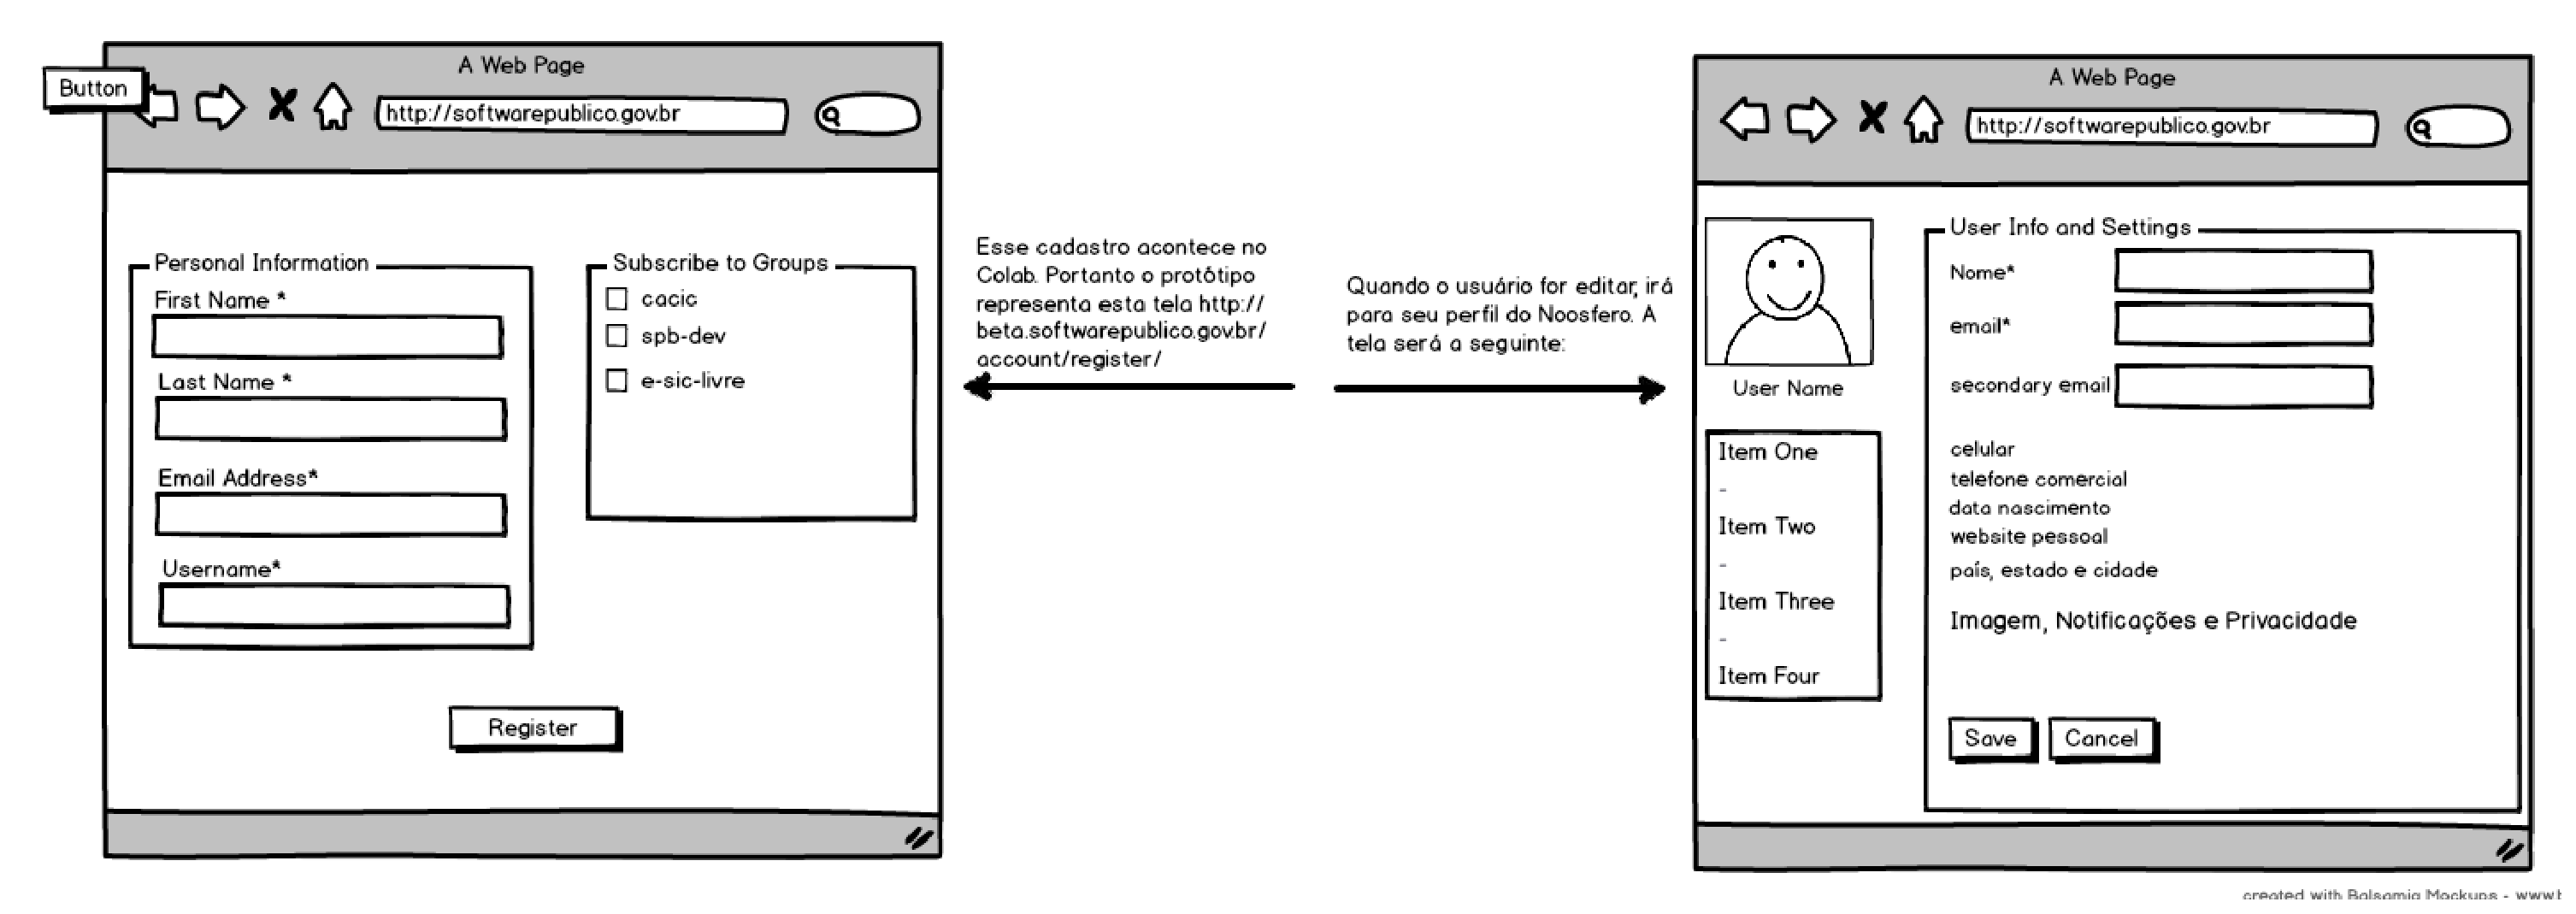
\includegraphics[keepaspectratio=true,scale=0.32]
      		{figuras/CadastroEdicaoUser.eps}
    	\caption{Protótipos de cadastro de usuário}
    	\label{cadastro user}
	\end{figure}

	\begin{figure}[h!]
    	\centering
    	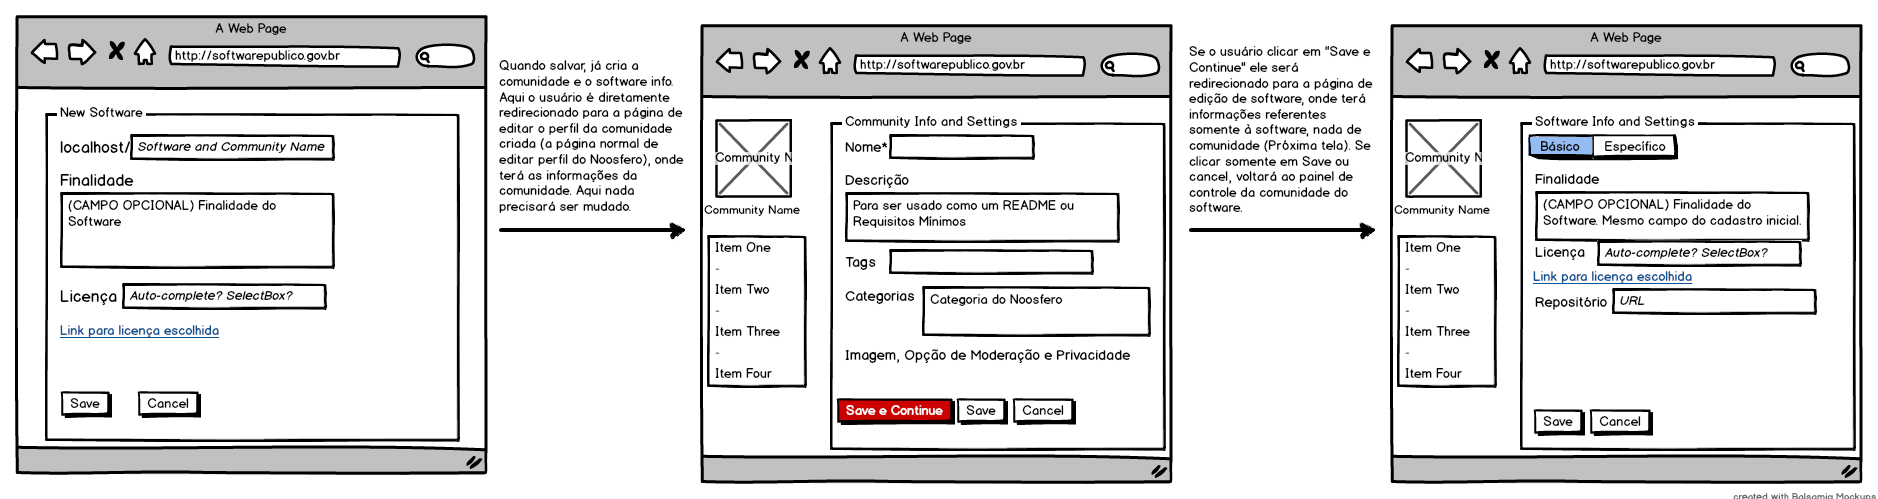
\includegraphics[keepaspectratio=true,scale=0.25]
      		{figuras/CadastroEdicaoSoftware.eps}
    	\caption{Protótipos de cadastro de software}
    	\label{cadastro software}
	\end{figure}

\newpage

\textbf{Cenários de Uso: }
	Para cada funcionalidade desenvolvida é determinado um cenário de uso, base para a implementação dos testes de aceitação e consequentemente o desenvolvimento da funcionalidade propriamente dita.
	Durante a primeira release (release 0) foram desenvolvidas algumas histórias, dentre estas, a história de ``Cadastro de Usuário'', que possui os seguintes cenários de sucesso:

	\begin{itemize}
	\item\textbf{Cenário 01:} Cadastro com sucesso de apenas campos obrigatórios

	\textbf{[Dado]} que não existe nenhum usuário com o nome de usuário ``josesilva''

	\textbf{[Quando]} eu clicar em cadastrar novo usuário

	\textbf{[E]} eu preencho os seguintes campos: 

  		\subitem nome de usuário: ``josesilva''

  		\subitem e-mail: ``jose@gmail.com''

  		\subitem senha: ``123456''

  		\subitem confirmação da senha: ``123456''

  		\subitem nome completo: ``José da Silva''

  		\subitem país: ``Brasil''

  		\subitem estado: ``Distrito Federal''

  		\subitem cidade: ``Brasília''

	\textbf{[E]} eu clico em cadastrar

	\textbf{[Então]} eu recebo uma confirmação de cadastro realizado com sucesso


	\item\textbf{Cenário 02:} Cadastro com sucesso de apenas campos obrigatórios de usuário governamental
	
	\textbf{[Dado]} que não existe nenhum usuário com o nome de usuário ``josesilva''
	
	\textbf{[Quando]} eu clicar em cadastrar novo usuário
	
	\textbf{[E]} eu preencho os seguintes campos: 
  		\subitem nome de usuário: ``josesilva''

  		\subitem e-mail: ``jose@serpro.gov.br''

  		\subitem e-mail secundário: ``jose@gmail.com''
j
  		\subitem senha: ``123456''

		\subitem confirmação da senha: ``123456''

		\subitem nome completo: ``José da Silva''

		\subitem cargo: ``analista de TI''

		\subitem país: ``Brasil''

		 \subitem estado: ``Distrito Federal''

		\subitem cidade: ``Brasília''

	\textbf{[E]} eu seleciono ``SERPRO'' como instituição

	\textbf{[E]} eu seleciono ``????'' como unidade  

	\textbf{[E]} eu clico em cadastrar

	\textbf{[Então]}eu recebo uma confirmação de cadastro realizado com sucesso

\item\textbf{Cenário 3:} Cadastro com sucesso com todos os campos preenchidos, mesmo não obrigatórios

	\textbf{[Dado]} que não existe um usuário cujo email primário ou email secundário é ``maria@gmail.com''

	\textbf{[Quando]} eu clicar em cadastrar novo usuário

	\textbf{[E]} eu preencho os seguintes campos: 

  		\subitem nome de usuário: ``mariasilva''

		  \subitem e-mail: ``maria@gmail.com''

		  \subitem e-mail secundário: ``maria@yahoo.com''

		  \subitem senha: ``123456''

		  \subitem confirmação da senha: ``123456''

		  \subitem nome completo: ``Maria da Silva''

		  \subitem cargo: ``analista de TI''

		  \subitem áreas de interesse: ``Engenharia de Software''

		  \subitem país: ``Brasil''

		  \subitem estado: ``Distrito Federal''

		  \subitem cidade: ``Brasília''

	\textbf{[E]} eu seleciono ``Outro'' como instituição 

	\textbf{[E]} eu clico em cadastrar

	\textbf{[Então]} eu recebo uma notificação de cadastro realizado com sucesso.
	\end{itemize}

	Os cenários de falha ocorrem nas seguintes situações:
	\begin{itemize}
	\item Email proposto existir como email de outro usuário;
	\item Email secundário proposto existir como email de outro usuário;
	\item Email secundário ser um email governamental e ao email primário não ser um email governamental;
	\item Não preenchimento de campos obrigatórios para usuário governamental 
	\end{itemize}
%Especificar as datas, as atividades realizadas.


Outra funcionalidade desenvolvida foi a história chamada ``Manter Instituição'', que possui os seguintes cenários:

\begin{itemize}
\item\textbf{Cenário 01:} Cadastro de nova instituição com sucesso

\textbf{[Dado]} que eu estou na página de cadastro de usuário

\textbf{[E]} que a seguinte instituição não existe:

  	\subitem nome: ``Ministério do Planejamento, Orçamento e Gestão''

  	\subitem sigla: ``MP''

 	\subitem poder: ``executivo''

 	\subitem esfera: ``federal''

  	\subitem tipo: ``pública''

  	\subitem cnpj: ``00.489.828/0002-36''

\textbf{[Quando]} eu clicar em ``Cadastrar nova instituição''

\textbf{[E]} eu preencher os seguintes campos:

  	\subitem sigla: ``MP''

  	\subitem poder: ``executivo''

  	\subitem esfera: ``federal''

  	\subitem tipo: ``pública''

  	\subitem cnpj: ``00.489.828/0002-36''

\textbf{[Então]} eu devo visualizar a mensagem ``Instituição cadastrada com sucesso!''

\item\textbf{Cenário 02:} Busca de instituição inexistente

\textbf{[Dado]} que eu estou na página de cadastro de usuário

\textbf{[E]} que a seguinte instituição não existe:

 \subitem nome: ``Ministério do Planejamento, Orçamento e Gestão''

  \subitem sigla: ``MP''

  \subitem poder: ``executivo''

  \subitem esfera: ``federal''

  \subitem tipo: ``pública''
  
  \subitem cnpj: ``00.489.828/0002-36''

\textbf{[Quando]} eu buscar MP

\textbf{[Então]} eu devo visualizar a mensagem ``Instituição não cadastrada''

\textbf{[E]}eu devo visualizar a opção de cadastrar nova instituição
\end{itemize}

Estes cenários apresentam alguns problemas de usabilidade analisando-os de acordo com as heurísticas de Nielsen, e após o processo de desenvolvimento ter uma melhoria na visão de usabilidade após a incorporação de profissionais da área, os cenários apresentaram melhoras em relação às heurísticas de Nielsen. 

Durante a segunda release (release 1) as histórias de ``Cadastro de Usuário'', e ``Manter Instituição'' foram desenvolvidas novamente com os seguintes cenários:

\begin{itemize}
\item\textbf{Cenário 01:} Cadastro com sucesso de apenas campos obrigatórios

	\textbf{[Dado]} que não existe nenhum usuário com o nome de usuário ``josesilva''

	\textbf{[Quando]} eu clicar em ``Cadastre-se''

	\textbf{[E]} eu preencho os seguintes campos: 

  		\subitem primeiro nome: ``José''

  		\subitem ultimo nome: ``Silva''

  		\subitem endereço de e-mail: ``jose@gmail.com''

  		\subitem usuário: ``josesilva''
  		
	\textbf{[E]} eu clico em ``Cadastre-se''

	\textbf{[Então]} eu recebo uma confirmação de cadastro realizado com sucesso, com a seguinte mensagem: 
	``Você deve se logar para seu perfil. Perfis não validados serão deletados em 24h.''
\end{itemize}

Para dar continuidade a este processo este estudo de caso avaliou os cenários estabelecidos e suas evoluções, verificando e propondo melhorias.

Durante a segunda release (release 2) a história de ``Novo Software'' foi desenvolvida com os seguintes cenários:

\begin{itemize}
\item\textbf{Cenário 01:} Novo Software

	\textbf{[Dado]} que não existe nenhum software com o localhost ``software''

	\textbf{[Quando]} eu clicar em ``Novo Software''

	\textbf{[E]} eu preencho os seguintes campos: 

  		\subitem localhost: ``software''

  		\subitem finalidade: ``Finalidade do software''

  		\subitem licenca: ``licença''
  		
  		
	\textbf{[E]} eu clico em ``Salvar''

	\textbf{[Então]} eu recebo uma confirmação de cadastro realizado com sucesso, e encontro a pagina de edição de software


Outros cenários de edição de software são: ``Informações de Comunidade'' e ``Informações de Software''.

\item\textbf{Cenário 02:} Informações de Comunidade

	\textbf{[Dado]} que ``software'' está cadastrado

	\textbf{[Quando]} eu clicar em ``Cadastre-se''

	\textbf{[E]} eu preencho os seguintes campos: 

  		\subitem descricao: ``Descrição do software''

  		\subitem tags: ``software''

  		\subitem categorias: ``categoria1''
 
	\textbf{[E]} eu clico em ``Salvar''

	\textbf{[Então]} eu recebo uma confirmação de cadastro salvo com sucesso


\item\textbf{Cenário 03:} Informações de Software

	\textbf{[Dado]} que ``software'' está cadastrado e estou em Edição de software

	\textbf{[Quando]} eu clicar em ``Especifico''

	\textbf{[E]} eu preencho os seguintes campos: 

  		\subitem Sigla: ``teste''

  		\subitem sistema operacional: ``teste os''

  		\subitem funcionalidades: ``testes''

  		\subitem categorias: ``categoria1''
 	
 	\textbf{[E]} eu clico em ``Nova Biblioteca''

 	\textbf{[E]} eu preencho os seguintes campos: 

 		\subitem nome: ``teste''

 		\subitem versão: ``teste''

 		\subitem licença: ``teste''

 	\textbf{[E]} eu clico em ``Novo Sistema Operacional''

 	\textbf{[E]} eu preencho os seguintes campos: 

 		\subitem nome: ``Debian''

 		\subitem versão: ``teste''

 	\textbf{[E]} eu clico em ``Nova linguagem''

 	\textbf{[E]} eu preencho os seguintes campos: 

 		\subitem nome: ``C++''

 		\subitem versão: ``teste''

 		\subitem sistema operacional: ``Debian''

 	\textbf{[E]} eu clico em ``Novo Banco de Dados''

 	\textbf{[E]} eu preencho os seguintes campos: 

 		\subitem nome: ``apache''

 		\subitem versão: ``teste''

 		\subitem sistema operacional: ``Debian''

	\textbf{[E]} eu clico em ``Salvar''

	\textbf{[Então]} eu recebo uma confirmação de cadastro salvo com sucesso
	
	
\end{itemize}

\textbf{Testes de Aceitação}

Os testes de aceitação software público são responsáveis por verificar os seguintes fatores:

\begin{itemize}
	\item Capacidade de registrar e editar informações de usuário e instituição;
	\item Capacidade de registrar e editar informações de software;
	\item Capacidade de desativar usuário;
	\item Capacidade de desativar software;
\end{itemize}


Segue abaixo os testes de aceitação desenvolvidos para e edição de software:

\textbf{Feature:} software registration
  As a user
  I want to create a new software
  So that I can have software communities on my network

  \textbf{Background:}

    \textbf{Given} ``MpogSoftwarePlugin'' plugin is enabled
  
    \textbf{And} SoftwareInfo has initial default values on database
  
    \textbf{And} I am logged in as admin
  
    \textbf{And} I go to /admin/plugins
  
    \textbf{And} I check ``MpogSoftwarePlugin''
  
    \textbf{And} I press ``Save changes''

  \textbf{Scenario:} Show library fields when click in New Library
  
    \textbf{Given} I go to admin user's control panel
  
    \textbf{And} I follow ``Manage my groups''
  
    \textbf{And} I follow ``Create a new software''
  
    \textbf{And} I follow ``New Library''
  
    \textbf{Then} I should see ``Name''
  
    \textbf{Then} I should see ``Version''
  
    \textbf{Then} I should see ``License''

  
  \textbf{Scenario:} Show SoftwareLangue fields when click in New Language
  
    \textbf{Given} I go to admin user's control panel
  
    \textbf{And} I follow ``Manage my groups''
  
    \textbf{And} I follow ``Create a new software''
  
    \textbf{And} I follow ``New language''
  
    \textbf{And} I should see ``3'' of this selector ``.software-language-table''
  
    \textbf{And} I follow ``Delete''
  
    \textbf{Then} I should see ``2'' of this selector ``.software-language-table''
    

 
  \textbf{Scenario:} Show databasefields when click in New database
  
    \textbf{Given} I go to admin user's control panel
  
     \textbf{And} I follow ``Create a new software''
  
     \textbf{And} I follow ``Manage my groups''
  
     \textbf{And} I follow ``New Database''
  
     \textbf{And} I should see ``3'' of this selector ``.database-table''
  
     \textbf{And} I follow ``Delete''
  
    \textbf{Then} I should see ``2'' of this selector ``.database-table''
   

  
  \textbf{Scenario}: Delete software libraries
  
    \textbf{Given} I go to admin user's control panel
  
    \textbf{And} I follow ``Manage my groups''
  
    \textbf{And} I follow ``Create a new software''
  
    \textbf{And} I follow ``New Library''
  
    \textbf{And} I should see ``2'' of this selector ``.library-table''
  
    \textbf{And} I follow ``Delete''
  
   \textbf{Then} I should see ``1'' of this selector ``.library-table''

Além dos testes de registro de software, também temos os testes de aceitação de registro de instituição:

Feature: Institution Field
  As a user
  I want to sign up resgistring my institution
  So others users can use it

  Background:
    \textbf{Given} ``MpogSoftwarePlugin'' plugin is enabled
    
    \textbf{And} I am logged in as admin
    
    \textbf{And} I go to /admin/plugins
    
    \textbf{And} I check ``MpogSoftwarePlugin''
    
    \textbf{And} I press ``Save changes''
    
    \textbf{And} I go to /account/logout
    
    \textbf{And} Institutions has initial default values on database

  
   \textbf{Scenario:} Show new institution fields when private institution is selected
    
    \textbf{Given} I go to /account/signup
    
    \textbf{When} I follow ``Create new institution''
    
    \textbf{And }I should see ``New Institution''
    
    \textbf{And }I should see ``Name''
    
    \textbf{And }I should see ``State''
    
    \textbf{And }I should see ``City''
    
    \textbf{And }I should see ``Country''
    
    \textbf{And }I should see ``CNPJ''
    
    \textbf{And }I should see ``Private Institution''

    \textbf{And }I choose ``Private Institution''
    
    \textbf{Then} I should see ``Fantasy name''


  
  \textbf{Scenario:} Create new public institution when all required fields are filled.

    \textbf{Given} I go to /account/signup

    \textbf{When} I follow ``Create new institution''

    \textbf{And }I fill in ``community name'' with ``Institution Name''

    \textbf{And }I fill in ``institutions cnpj'' with ``00.000.000/0001-00''

    \textbf{And }I select ``Brazil'' from ``community country''

    \textbf{And }I fill in ``community state'' with ``DF''

    \textbf{And }I fill in ``community city'' with ``Brasilia''

    \textbf{And }I choose ``Public Institution''

    \textbf{And }I select ``Executivo'' from ``institutions governmental power''

    \textbf{And }I select ``Federal'' from ``institutions governmental sphere''

    \textbf{And }I select ``Autarquia'' from ``institutions juridical nature''

    \textbf{And }I follow ``Save''

    \textbf{Then} I should see ``Institution Name''


  
  \textbf{Scenario:} Create new private institution when all required fields are filled

    \textbf{Given} I go to /account/signup

    \textbf{When} I follow ``Create new institution''

    \textbf{And }I fill in ``community name'' with ``Institution Name''

    \textbf{And }I fill in ``institutions cnpj'' with ``00.000.000/0001-00''

    \textbf{And }I select ``Brazil'' from ``community country''

    \textbf{And }I fill in ``community state'' with ``DF''

    \textbf{And }I fill in ``community city'' with ``Brasilia''

    \textbf{And }I choose ``Private Institution''

    \textbf{And }I follow ``Save''

    \textbf{Then} I should see ``Institution Name''

      
  
  \textbf{Scenario:} Don't create an institution when name and cpnj are not filled

    \textbf{Given} I go to /account/signup

    \textbf{When} I follow ``Create new institution''

    \textbf{And }I choose ``Private Institution''

    \textbf{And }I fill in ``institutions acronym'' with ``Teste''

    \textbf{And }I select ``Brazil'' from ``community country''

    \textbf{And }I fill in ``community state'' with ``DF''

    \textbf{And }I fill in ``community city'' with ``Brasilia''

    \textbf{And }I follow ``Save''

    \textbf{Then} I should see ``Institution could not be created!''

    \textbf{And }I should see ``Name can't be blank''

    \textbf{And }I should see ``CNPJ can't be blank''



  \textbf{Scenario:} Don't Create new institution when a governamental field is not filled

    \textbf{Given} I go to /account/signup

    \textbf{When} I follow ``Create new institution''

    \textbf{And }I fill in ``community name'' with ``Institution Name''

    \textbf{And }I fill in ``institutions cnpj'' with ``00.000.000/0001-00''

    \textbf{And }I select ``Brazil'' from ``community country''

    \textbf{And }I fill in ``community state'' with ``DF''

    \textbf{And }I fill in ``community city'' with ``Brasilia''

    \textbf{And }I choose ``Public Institution"

    \textbf{And }I follow ``Save''

    \textbf{Then} I should see ``Governmental power can't be blank''

    \textbf{And }I should see ``Governmental sphere can't be blank''

    \textbf{And }I should see ``Juridical nature can't be blank''


\subsection{Testes com usuários}
	
	\textbf{Objetivos}
	
		O objetivo do teste com os usuários é ter um feedback das funcionalidades a fim de capturar problemas de usabilidade. 
	
	\textbf{Tarefas}

	Primeiramente foi identificada algumas tarefas que devem podem ser executadas com as funcionalidades desenvolvidas no portal até o exato momento.
	
	\begin{itemize}
	
		\item Cadastrar um novo usuário no Portal.
		\item Editar seu perfil de usuário.
		\item Cadastrar uma nova instituição.
		\item Cadastrar um novo software no Portal do Software Público.
		\item Cadastrar Comunidade relacionado ao novo software
		\item Editar informações do software.
		\item Editar informações do usuário.
		
	\end{itemize}
	
	Depois de especificado as tarefas que podem ser executados, foram escritos script que o usuário possa seguir:
	
	\textbf{Scripts}%alterei o nome pra nao confundir o leitor;

	\begin{itemize}
	
		\item ``Você é um representante de uma comunidade de software livre e descobriu que existe o portal do Software Público Brasileiro e deseja cadastrar o software no Portal''.

	\end{itemize}
			
	\textbf{Teste Piloto}
	
	Com teste piloto, escolhemos um membro da equipe que não tinha participado do desenvolvimento da funcionalidade para testar os scripts e tarefas. %A pessoa a ser testada também faz parte do grupo de usuários do sistema.
	
	\textbf{Observação}
	
		A observação permite que o avaliador tenha uma visão dos problemas sendo vivenciados pelos usuários. É importante observar o que o usuário está fazendo e realizar as anotações. %Também pode ser gravado o áudio ou a tela do usuário. Neste caso optamos por não gravar a tela do usuário.
	

\section{Análise e Interpretação dos Resultados}

Esta seção apresenta a discussão e a interpretação dos resultados observados durante a execução do estudo de caso descrito.

Analisando os protótipos e os cenários desenvolvidos, de acordo com as heurísticas de Nielsen, encontramos alguns problemas de usabilidade e propomos tarefas de melhorias a serem feitas e possivelmente verificadas durante os testes de aceitação.


\subsection{Análise dos Dados}

A partir dos protótipos e dos cenários desenvolvidos durante as releases 0 e 1, analisamos alguns problemas de usabilidade com base nas heurísticas de Nielsen. A tabela abaixo descreve os problemas encontrados nas primeiras análises.

A partir do levantamento desses problemas foram propostas tarefas durante o planejamento de atividades da equipe de desenvolvimento, para que assim cada problema pudesse ser discutido e resolvido.

\newpage

\begin{table}[h!]
\begin{tabular}{|l|p{3cm}|p{6cm}|p{3cm}|l|}
\hline
\textbf{ID} & \textbf{Local} & \textbf{Descrição do Problema}                                                                                     & \textbf{Heurística Desobedecida} & \textbf{Criticidade} \\ \hline
1           & Protótipo - Novo Software                 & Ao escolher um nome para o software, não há evidência do que aconteceria caso o nome fosse igual a outro existente & Prevenção de erros               & Média                \\ \hline
2           & Protótipo - Novo Software                 & Não há informação para o usuário do que seria o ``Link''                                                             & Ajuda e documentação             & Média                \\ \hline
3           & Protótipo - Nova Comunidade               & Palavras em inglês e português                                                                                     & Linguagem Clara                   & Baixa                \\ \hline
4           & Protótipo - Nova Comunidade               & Falta de informação sobre as tags e as categorias do noosfero                                                      & Ajuda e documentação             & Baixa                \\ \hline
5           & Protótipo - Novo Software                 & Campos obrigatórios não são definidos                                                                              & Prevenção de erros               & Média                \\ \hline
6           & Protótipo - Novo Software    & Mensagens de ajuda ao preenchimentos dos campos                                                                    & Prevenção de erros               & Baixa                \\ \hline
7           & Protótipo - Nova Comunidade               & Botão de Save e Continue altera estrutura da pagina de software                                                    & Consistência                     & Baixa                \\ \hline
\end{tabular}
\end{table}

\newpage

\begin{table}[h!]
\begin{tabular}{|l|p{3cm}|p{6cm}|p{3cm}|l|}
\hline
\textbf{ID} & \textbf{Local} & \textbf{Descrição do Problema}                                                                                     & \textbf{Heurística Desobedecida} & \textbf{Criticidade} \\ \hline
1           & Cadastro de Usuário                 & Linguagens estrangeiras e avisos em outros idiomas & Diálogos simples  & Média                \\ \hline
2           & Cadastro de Usuário      & Botão de adicionar nova instituição não é claro para o usuário.  & Minimizar a sobrecarga de memória do usuário;           & Alta                \\ \hline
3           & Cadastro de Usuário               & Diferença entre botão adicionar nova instituição e criar nova instituição para o usuário  & Minimizar a sobrecarga de memória do usuário & Media                \\ \hline
4           & Cadastro de Instituição             & Seleção de País deve ter Brasil como default  & Diálogos simples e naturais    & Baixa                \\ \hline
5           & Cadastro de Instituição      & Opção de escolha do estado: Random button não posicionado e não funciona no primeiro clique. & Diálogos simples e naturais  & Baixa                \\ \hline
6           & Cadastro de Usuário  & Caso você não preencha o email secundário ele informa a seguinte mensagem: E-mail or secondary e-mail already taken & Boas mensagens de erros                & Média                \\ \hline
7           & Cadastro de Usuário  & Opção recaptcha só aparece na segunda vez & Consistência                     & Alta                \\ \hline
8           & Perfil de Usuário  & Ao clicar em hide no bloco de progresso de perfil ele some e não foi encontrada uma opção fácil para reverter a situação.
 & Prevenção de erros                     & Baixa                \\ \hline
9           & Cadastro de Usuário  & Caso se tenha uma infinidade de grupos, fica inviável a opção de checkbox. Ou será utilizada apenas para grupos mais ``conhecidos''? & Atalhos & Média                \\ \hline
10           & Cadastro de Usuário  & Mensagem de erro um pouco confusa: Usuário com este Usuário já existe.  & Consistência                     & Baixa                \\ \hline
\end{tabular}
\end{table}

\newpage
No segundo ciclo de avaliações levantamos os seguintes problemas em relação as histórias de ``Cadastro de Usuário'' e ``Cadastro de Software'':

\begin{table}[h!]
\begin{tabular}{|l|p{3cm}|p{6cm}|p{3cm}|l|}
\hline
\textbf{ID} & \textbf{Local} & \textbf{Descrição do Problema}                                                                                     & \textbf{Heurística Desobedecida} & \textbf{Criticidade} \\ \hline
1           & Cadastro de Usuário                 & Rótulos dos campos de registro não contém um elemento de convite à entrada de dados ( “ : ”) & Diálogos simples e naturais     & Baixa                \\ \hline
2           & Cadastro de Usuário                 & Usuário não encontra informações suficientes sobre grupos que pode participar  & Diálogos simples e naturais             & Média                \\ \hline
3           & Cadastro de Usuário               & Ao se excluir um e-mail secundário, não existe solicitação de confirmação       & Feedback                & Alta                \\ \hline
4           & Cadastro de Software      & Dificuldade para acessar o botão de criar software
	        & Minimizar sobrecarga          & Baixa                \\ \hline
5           & Cadastro de Software       & Funcionalidade de criar software também cria comunidade, porém o usuário não é informado disto  & Feedback    & Média                \\ \hline
6           & Cadastro de Software    & Dificuldade para acessar o botão de editar software
		    & Minimizar sobrecarga           & Baixa                \\ \hline
7           & Cadastro de Software    & Fluxo de edição não está claro (etapas)
			& Feedback                       & Média                \\ \hline
8           & Cadastro de Software    & frase ``The highlighted fields are mandatory'' não especifica o char (*)
		    &Diálogos simples e naturais     & Baixa                \\ \hline
\end{tabular}
\end{table}

 

\newpage


\subsection{Análise dos Resultados de Medição}
\label{analise}
Analisando os dados das primeiras releases, que compõem o primeiro ciclo de avaliações pelas heurísticas. No segundo ciclo de avaliações usamos os \textit{checklists} em \ref{checklists} desenvolvidos para auxiliar as avaliações das heurísticas, também utilizados no terceiro ciclo de avaliações. Uma das histórias avaliadas foi a de ``Cadastro de Usuário'':

\begin{figure}[h!]
    	\centering
    	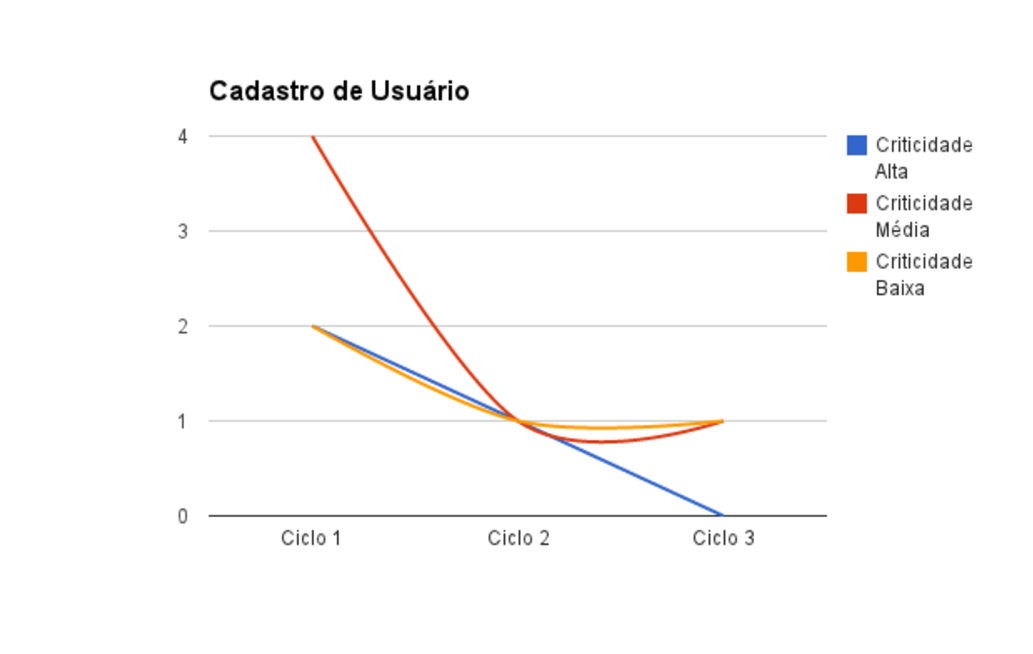
\includegraphics[keepaspectratio=true,scale=0.62]
      		{figuras/graf01.eps}
    	\caption{Resultado das avaliações de ``Cadastro de Usuário''}
    	\label{avaliacaouser}
\end{figure}

Já em ``Cadastro de Instituição'', temos:

\begin{figure}[h!]
    	\centering
    	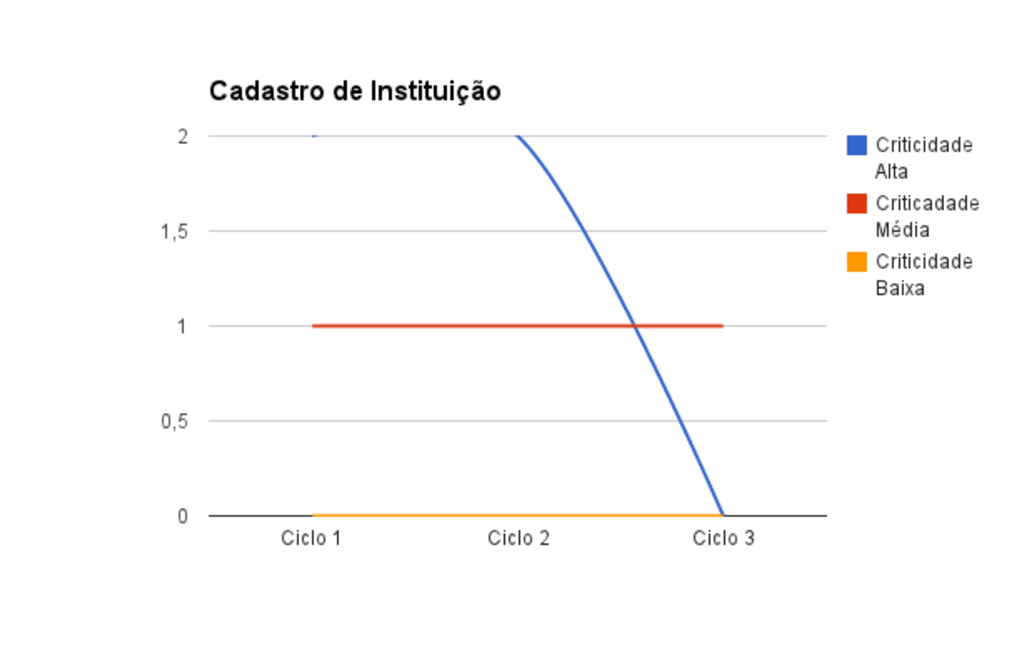
\includegraphics[keepaspectratio=true,scale=0.62]
      		{figuras/graf02.eps}
    	\caption{Resultado das avaliações de ``Cadastro de Instituição''}
    	\label{avaliacaoinstitucion}
\end{figure}

Quanto à história de ``Cadastro de  Software'', temos:

\begin{figure}[h!]
    	\centering
    	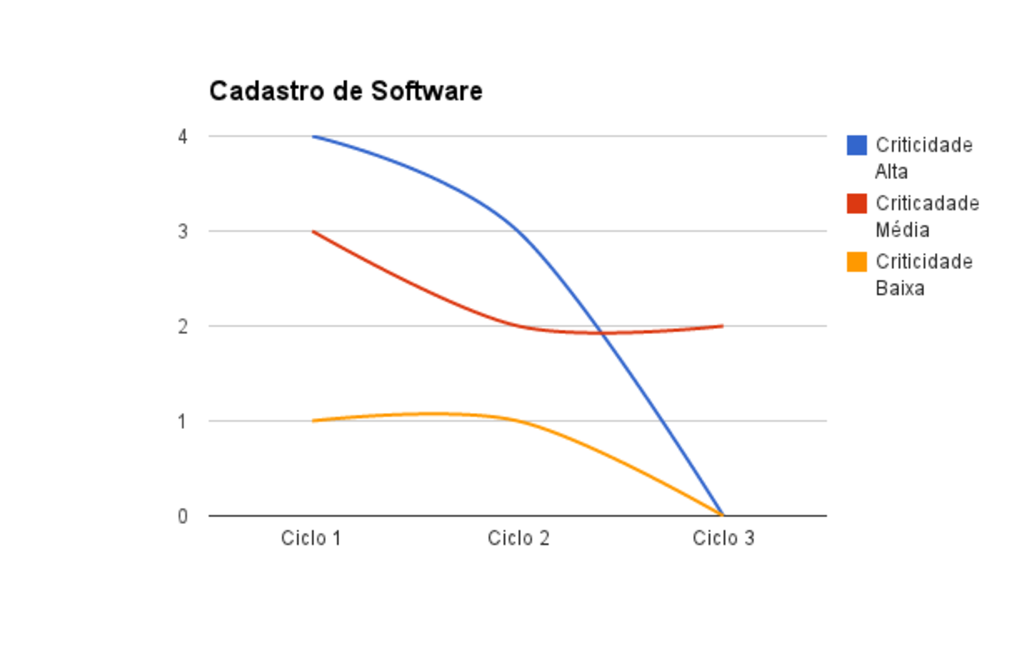
\includegraphics[keepaspectratio=true,scale=0.62]
      		{figuras/graf03.eps}
    	\caption{Resultado das avaliações de ``Cadastro de Software''}
    	\label{avaliacaosoftware}
\end{figure}

\begin{comment}

Analisando os dados das primeiras releases, que compõem o primeiro ciclo de avaliações pelas heurísticas temos em ``Cadastro de Usuário'':
\begin{itemize}
	\item 2 problemas de criticidade baixa;
	\item 4 problemas de criticidade média;
	\item 2 problemas de criticidade alta;
\end{itemize}

Já em ``Cadastro de Instituição'', temos:
\begin{itemize}
	\item 2 problemas de criticidade baixa;
	\item 0 problemas de criticidade média;
	\item 0 problemas de criticidade alta;
\end{itemize}

Quanto à história de ``Cadastro de  Software'', temos:
\begin{itemize}
	\item 4 problemas de criticidade baixa;
	\item 3 problemas de criticidade média;
	\item 0 problemas de criticidade alta;
\end{itemize}

No segundo ciclo de avaliações usamos os \textit{checklists} em \ref{checklists} desenvolvidos para auxiliar as avaliações das heurísticas. Uma das histórias avaliadas foi a de ``Cadastro de Usuário'':

\begin{itemize}
	\item 1 problema de criticidade baixa;
	\item 1 problema de criticidade média;
	\item 1 problema de criticidade alta;
\end{itemize} 



Outra história avaliada nesta segunda rodada foi a de ``Cadastro de Software'':

\begin{itemize}
	\item 3 problemas de criticidade baixa;
	\item 2 problemas de criticidade média;
	\item 0 problemas de criticidade alta;
\end{itemize} 
\end{comment}

\newpage
Quanto aos testes de aceitação dos cenários avaliados tivemos os seguintes resultados de medição:

História: ``Cadastro de Usuário'':
\begin{itemize}
	\item Quantidade de cenários executados: 22 cenários;
	\item Quantidade de passos executadas: 162 passos
	\item Quantidade de falhas obtidas: 0 falhas;
\end{itemize} 

História: ``Cadastro de Software'':
\begin{itemize}
	\item Quantidade de cenários executados: 6 cenários;
	\item Quantidade de passos executadas: 68 passos
	\item Quantidade de falhas obtidas: 0 falhas;
\end{itemize} 

\subsection{Verificação}

Esta subseção analisa os verifica alcançados no estudo de caso, baseado na hipótese levantada e apresentada no início desta seção. Podemos ver nas figuras \ref{avaliacaouser}, \ref{avaliacaoinstitucion} e \ref{avaliacaosoftware} que a partir das avaliações de heurísticas nos protótipos e cenários diminuiu ou se manteve o numero de casos com problemas de criticidade alta, média ou baixa. 

\subsection{Observações acerca das técnicas utilizadas e planejadas}

	Nessa subseção relatamos alguns pontos que identificamos ao adotar algumas técnicas e métodos de usabilidade no ciclo de desenvolvimento do projeto.

	\textbf{Questionários de Perfil de Uso:}

	A aplicação de questionários de perfil de usuário antes e durante a produção do sistema é importante para entender as principais necessidades do público alvo. Se um questionário for aplicado e não for utilizado como insumo para o desenvolvimento do sistema, ele perde o sentido de ser realizado, pois não trará nenhum beneficío ao desenvolvimento/design do sistema, apenas servirá como arcabouço teórico para futuras avaliações, deixando de lado a questão do design centrado no usuário.

	\textbf{Histórias de Usabilidade}

	No contexto do desenvolvimento ágil, as histórias de usabilidade apoiadas pela criação de Persona e Roteiros podem ser uma das melhores técnicas para inserir práticas de usabilidade no inicio do ciclo de desenvolvimento ágil de software pois são comparadas com as histórias de usuário utilizadas no desenvolvimento empírico. 

	\textbf{Perfil do Usuário}

	A determinação do perfil do usuário é extremamente importante para o sucesso do projeto e do teste, pois um mesmo sistema pode ser excelente para algumas pessoas e inadequado ou inaceitável para outras. Para se criar um cenário de teste é importante ter em mente quem são os possíveis usuários.

	%\textbf{Avaliação Heurística}
	
	%Um dos problemas encontrados na utilização da técnica de avaliação heurística dentro de uma equipe de desenvolvimento empírico, muitas vezes é devido que nem sempre há especialistas em usabilidade integrantes na equipe para realizar uma avaliação sistemática do sistema à ser desenvolvido.

	%Obs: existem especialistas no spb, essa observação tá errada.
	
	\textbf{Checklist}
	
	A utilização checklists no contexto de uma equipe de desenvolvimento de software é mais prático pois existem ferramentas que auxiliam na condução de um checklist de usabilidade, como por exemplo o Ergolist.

	\textbf{Design Centrado no usuário}
	
	Para que um projeto seja centrado no usuário, é importante que o usuário seja inserido do início ao fim do processo. 
	

\section{Considerações finais do capítulo}

Este capítulo apresentou o estudo de caso sobre o desenvolvimento do Portal do Software Público a partir de métodos empíricos, utilizando práticas de BDD e usabilidade.







